%!TEX root = ../thesis.tex
%*******************************************************************************
%*********************************** First Chapter *****************************
%*******************************************************************************
\chapter{Markov Processes}  %Title of the First Chapter

\ifpdf%
    \graphicspath{{Chapter1/Figs/Raster/}{Chapter1/Figs/PDF/}{Chapter1/Figs/}}
\else
    \graphicspath{{Chapter1/Figs/Vector/}{Chapter1/Figs/}}
\fi

\tikzstyle{state}=[shape=circle,draw=blue!50,fill=blue!20]
\tikzstyle{observation}=[shape=rectangle,draw=orange!50,fill=orange!20]
\tikzstyle{lightedge}=[<-,dotted]
\tikzstyle{mainstate}=[state,thick]
\tikzstyle{mainedge}=[<-,thick]

At its core, a Markov chain is a stochastic model describing a sequence of possible events where the probability of each event depends solely on the state attained in the previous event. This is termed as the 'Markov Property', which encapsulates the memorylessness of the process — the future is independent of the past given the present.

Markov chains provide a robust framework for modeling the probabilistic nature of cryptocurrency markets. The rapid fluctuation of cryptocurrency prices, driven by a myriad of factors such as market sentiment, technological advancements, regulatory news, and macroeconomic trends, can be represented effectively using Markov chains.

In this chapter, we start by laying down the fundamental theoretical foundations of Markov chains. This includes an explanation of key concepts such as state spaces, transition probabilities, and the difference between discrete and continuous time Markov chains. Understanding these basic building blocks is pivotal in leveraging Markov chains for cryptocurrency market analysis.

Next, we focus on specific properties of Markov chains like irreducibility, periodicity, and stationarity, which play critical roles in determining the long-term behavior of the chain

%********************************** %First Section  **************************************
\section{Discrete-time Markov Chains} %Section - 1.2

Let $\Omega \neq \emptyset$ and $\mathcal{F} \subseteq 2^{\Omega}$ be a $\sigma$-algebra on $\Omega$, and $P$ a measure on A with $P(\Omega) = 1$, i.e. $P$ is a {\it probability measure}. Then the triplet $(\Omega, A, P)$ is called a {\it probability space}. Where $\Omega$ denotes a sure event, and it holds that $\forall \omega \in \Omega$ is called an elementary event. Furthermore, $\forall A \in A$ is a random event  so that $P(A)$ is a probability of such a random event. 

Let $I$ be a countable set and $\Theta$ a $\sigma$-algebra on $I$. Each $i \in I$ is called a \textit{state} and $(I,\Theta)$ a \textit{state-space}. We say that $\lambda = (\lambda_i : i \in I) $ is a measure on I if $0 \leq \lambda_i \leq \infty$. If in addition the {\it total mass} $\sum_{i \in I} \lambda_i = 1$ then $\lambda$ is a {\it distribution} (or probability measure). 

Suppose now that we have two measurable spaces $(\Omega,A)$ and $(I,\Theta)$ and a random variable $X: \Omega \rightarrow I$ assuming that X is measurable. Thus, we call $(I,\Theta)$ a state space and $(\Omega, A)$ an underlying space. Therefore, we may set:

\begin{equation}
\lambda_X(i) = P(X=i)=P(\{\omega: X(\omega)=i\})
\end{equation}

Since we are allowing only for the discrete realizations of the random variable X, given previous assumptions, $\lambda_X(i)$ is a {\it probability mass function}.

Then measure $\lambda$ defines a distribution of $X$. Given such a setting random variable $X$ is assumed to denote random state $i$ with probability $\lambda_i$. 

Let us now assume that we have a sequence of random variables $\{X_t : t \in T\}$ where $T$ is a countable set of time steps.
 We say that $\{X_t : t \in T\}$ is a {\it stochastic process} and if it also holds that $T = \mathbb{N}_0$ then {\it discrete-time stochastic process}.
 In the context of Markov Chains we call measurable space $I$ as a {\it state space} and $X_t$ as a {\it state} at time $t$ respectively.
 Given the initial setup, we may define a {\it discrete-time Markov Chain} as a stochastic process $\{X_t : t \in T\}$ with a state space $I$ and a distribution $\lambda$ such that for all $t \in T$ and $i_0,i_1,\ldots,i_{t+1} \in I$ it holds that:

\begin{equation} \label{DTMC}
P(X_{t+1}=i_{t+1}|X_t=i_t,\ldots,X_0=i_0) = P(X_{t+1}=i_{t+1}|X_t=i_t)
\end{equation}

which holds for all $t \in T$ and $i_0,i_1,\ldots,i_{t+1} \in I$. In other words, the probability of observing a state $i_{t+1}$ at time $t+1$ given the sequence of states $i_0,i_1,\ldots,i_{t+1}$ is equal to the probability of observing a state $i_{t+1}$ at time $t+1$ given only the last observed state $i_t$.
This fundamental relationship is called {\it Markov property}, and it is a consequence of the {\it memoryless property} of Markov Chains. 
Conditional property of Markov Chains may be equivalently expressed using current state as $i \in I$ and a previous state $j \in I$ as:

\begin{equation}
P(X_{t+1}=i|X_t=j) = p_{j,i}(t,t+1)
\end{equation}

where $p_{j,i}(t,t+1)$ is a {\it transition probability} from state $j$ to state $i$ at time $t$ and $t+1$ respectively. Sometimes we refer to these transitions as {\it one-step transitions} since they are only dependent on the previous state.
As an extension of the Markov property we may also define a {\it k-step transition} as a probability of observing a state $i$ at time $t+k$ given the state $j$ at time $t$ as:

\begin{equation}
P(X_{t+k}=i|X_t=j) = p_{j,i}(t,t+k)
\end{equation}

One important distinction is that if the transition probabilities $p_{j,i}(t,t+k)$ do not depend on time $t$ then the Markov Chain is called {\it homogeneous} otherwise these probabilities vary over time, therefore {\it heterogeneous} Markov Chain.
Considering only first order homogeneous Markov Chain we may define a {\it transition matrix} 
$A = (p_{i,j} : i,j \in I)$ as a matrix of transition probabilities between each state $i,j \in I$ such that:

\begin{equation} \label{eq:1.5}
p_{j,i} \geq 0 \quad i,j \in I; \quad \sum_{j \in I} ^{}p_{i,j} = 1, \quad \forall i \in I
\end{equation}

Rectangular matrix $P$ that satisfies property given by Equation \ref{eq:1.5} is called {\it stochastic matrix}. 
Furthermore, we ought to define a probability distribution $\textbf{p} =\{p_i, i \in I\} $ as a vector of probabilities of observing a each state at time $t=0$ such that:

\begin{equation}
p_i = P(X_0=i), \quad i \in I
\end{equation}

and 

\begin{equation}
p_i \geq 0 \quad i \in I; \quad \sum_{i \in I} ^{}p_i = 1
\end{equation}

which is also called \textit{initial distribution} of Markov Chain. 

According to~\cite{Praskova2012}, once we have transition matrix $A$ and initial distribution $\textbf{p}$ that satisfy constraints given by Equation (1.5) and (1.7) respectively,
then $\{X_t,t \in \mathbb{N}_0\}$ is a discrete-time homogeneous Markov Chain with transition matrix $A$ and initial distribution $\textbf{p}$ 
if and only if all finite dimensional distributions of $\{X_t,t \in \mathbb{N}_0\}$ are consistent with the following equation:

\begin{equation}
P(X_{0}=i_0,X_{1}=i_1,\ldots,X_{k}=i_k) = p_{i_0} p_{i_0,i_1} \ldots p_{i_{k-1},i_k}
\end{equation}

where $i_0,i_1,\ldots,i_k \in I$ and $k \in \mathbb{N}_0$. If we abstract from the initial distribution $p$, such equation is called \textit{Chapman-Kolmogorov equation} as in~\cite{Yin2004}.
Above stated equation also holds for non-homogeneous Markov Chains with the only difference that the transition probabilities $p_{i,j}$ are time dependent:

\begin{equation}
P(X_{0}=i_0,X_{1}=i_1,\ldots,X_{k}=i_k) = p_{i_0}(0) p_{i_0,i_1}(0,1) \ldots p_{i_{k-1},i_k}(k-1,k)
\end{equation}

another substantial property of homogeneous Markov Chains is that their nth order transition probabilities can be expressed as a product of first order transition probabilities:

\begin{equation}
P(X_{m+n} = j|X_{m} = i) = p_{i,j}^{(n)}, \quad i,j \in I
\end{equation}

where generally $p_{i,j}^{(m+n)} = \sum_{k \in I} p_{i,k}^{(m)} p_{k,j}^{(n)}$ is referred to as \textit{Chapman-Kolmogorov equality} and holds for $m,n \in \mathbb{N}_0$ and $P(X_m=i) \geq 0$.

To simply illustrate the idea behind discrete-time homogeneous Markov Chains let us assume a situation where the future market movements transition between a countable number of states $I =$ \{upward, side, downward\} 
and there is a transition matrix A and initial distribution $p$:
\begin{equation}
A =
\begin{pmatrix}
0.1 & 0.4 & 0.5 \\
0.25 & 0.3 & 0.45 \\
0.33 & 0.33 & 0.33 
\end{pmatrix} 
, \quad p = 
\begin{pmatrix}
    0.2 & 0.3 & 0.5 \\
\end{pmatrix}
\end{equation}



Each row represents full set of transition probabilities between states, also visible from $\sum_{j \in I} ^{}p_{i,j} = 1 $, i.e. each row of matrix $A$ represents a conditional probability distribution given $i \in I$. 
Such a relationship can be represented as a diagram indexing each state by U, S and D respectively as follows:

\begin{center}
\begin{tikzpicture}[->, >=stealth', auto, semithick, node distance=3cm]
\tikzstyle{every state}=[fill=white,draw=black,thick,text=black,scale=1]
\node[state]    (U)                     {$U$};
\node[state]    (S)[right of=U]   {$S$};
\node[state]    (D)[right of=S]   {$D$};

\path
(U) edge[loop left]     node{$0.1$}         (U)
    edge[bend left,below]     node{$0.4$}     (S)
    edge[bend right,below]      node{$0.5$}      (D)
(S) edge[bend left,below]     node{$0.45$}           (D)
    edge[loop below]     node{$0.3$}           (S)
    edge[bend left, above]     node{$0.25$}           (U)
(D) edge[bend right,above] node{$0.33$}           (U)
    edge[loop right]     node{$0.33$}         (D)
    edge[bend left, above]      node{$0.33$}         (S);
\end{tikzpicture}
\end{center}


 
This may be easily interpreted for each given state. For example if we assume that the market moved upwards on the last trading day there is a 0.1 chance that the market will move in positive direction today, in other words the conditional probability of observing the state U today given the state U yesterday is 0.1. 
On the hand if we suppose that today the market actually transitioned to the state S with probability 0.4 there is now a probability of 0.45 to transition to state D since the future transition is only conditioned by its previous state. 

Up until now we have assumed random variable X that modelled the probability of observing a state $i \in I$ given the initial distribution $\lambda$. We ought to consider  thus we have to allow for a system of discrete random variables that are also identically distributed for each time step $\{X_{t},t \in T \}$, for $\{t_0,t_1,\ldots,t_n\} \subset T$ where $n \in \mathbb{N}_0$.

Suppose now that we have observed a given sequence of states for the last week as $\{U,S,D,D,U\}$, and we would like to know the sequence joint probability given the transition matrix A and initial distribution $p$:

\begin{align*}
P(X_{t_0} = x_0,\ldots,X_{t_n} = x_n|A,p) &= P(X_0 = x_0) \prod_{k=1}^4 P(X_k=x_k|X_{k-1}=x_{k-1})\\
&= p_{x_0} p_{1,2}  p_{2,3}  p_{3,3} p_{3,1} \\
&= 0.2 * 0.4 * 0.45 * 0.33 * 0.33 \\
&= 0.002376
\end{align*}

Where the probability of observing state A is determined by our distribution $\lambda$ evaluated at respective state A since we have no prior knowledge about what exactly happened before $t_0$. 

On the other hand, we might consider a situation in which we have observed such a sequence of events, and we need to determine the next state given the sequence. As in the last example, we have our transition matrix P, distribution $\lambda$ and a sequence of events observed until now $\{A,B,C,C,A\}$ for $t_{k-4},\ldots,t_{k}$. Let us also assume that $t_{k+1}$ is a time of next event for which we are trying to determine its probability.

\begin{align}
P(X_{t_{k+1}}|X_{t_{k}},\ldots,X_{t_{k-4}}) &= P(X_{t_{k+1}}|X_{t_{k}})
\end{align}

We know that last observed state was $U$ which directs us straight to the first row of our transition matrix A since from the properties of Markov Processes we know that the next state will depend solely on the present state, 
so we can abstract from the given sequence of past states and focus only on $X_{t_{k}}$. Finally, we may conclude that the most likely future state at time $t_{k+1}$ is D with the probability of 0.5. Formally we may write:

\begin{equation}
 i_{k+1} = \underset{i \in I}{\arg\max} P(X_{t_{k+1}}=i_{k+1}|X_{t_{k}}=i_{k}) \\
\end{equation}

\subsection{Classification of states}

Markov Chains may be classified into several categories based on their properties. 
Firstly, we may distinguish between {\it transient} and {\it recurrent} states and as a convenient notation we will introduce so called {\it return time} $\tau_j$ 
as a random variable that denotes the time of kth return to state $j \in I$:

\begin{equation}
\tau_j(k+1) = \inf \{n \geq \tau_j(k) : X_n =j\}, \quad k \in \mathbb{N}_0
\end{equation}

if $\tau_j(k) \leq \infty$ and we assume that $\inf\{\emptyset\} = \infty$ and $\tau_j(0) = 0$.

This random variable also satisfies properties of {\it recurrence time}. 
Any random variable $\tau:\Omega \to \mathbb{N}_0 \cup \{ \infty \}$ for which outcomes $[\tau = n]$ belong to 
$\sigma$-algebra $\mathcal{F}_n = \sigma(X_0,\ldots,X_n)$ generated by random variables $X_0,X_1, \ldots , X_n$ is called a {\it recurrence time}.

A state $j \in I$ is called {\it transient} if there is a non-zero probability that the process will never return to state $j$ once it has left it, i.e.:

\begin{equation}
P(\tau_j(1) = \infty|X_0=j) > 0, \quad \sum_{n=0}^{\infty} p_{j,j}^{(n)} \leq \infty
\end{equation}

for some $k \in \mathbb{N}_0$. On the other hand, a state $j \in I$ is called {\it recurrent} if it is not transient, i.e.:

\begin{equation}
P(\tau_j(1) \leq \infty|X_0=j) = 1, \quad \sum_{n=0}^{\infty} p_{j,j}^{(n)} = \infty
\end{equation}

We can further distinguish between {\it positive recurrent} if the expected return time is finite $E[\tau_j(1)|X_0=j] < \infty$ and {\it null recurrent} if the expected return time is infinite $E[\tau_j(1)|X_0=j] = \infty$.

Let us make one more distinction regarding a Markov chain states. State is said to be periodic if it can only be revisited (i.e., return to the same state) in multiples of some integer larger than 1. 
The greatest common divisor of these numbers is the period. If the period is larger than 1, the state is called periodic and 
on the contrary, if there is no such integer and the state can be revisited at any time, then the state is called aperiodic. 
If all states in a Markov chain are aperiodic, the Markov chain itself is said to be aperiodic as well. Aperiodicity is a desirable property for a Markov chain because it ensures that the chain does not get trapped in oscillating sequences of states. 
To clarify, a periodicity does not mean that each state must be reachable from every other state in just one step. It's a more subtle concept, meaning that the greatest common divisor of the lengths of all cycles in the chain must be 1, so that any state can be reached from any other state in a variable number of steps.
Previous properties of states lead us to define ergodic state for which it holds that it needs to be positive recurrent and aperiodic. Such trait is desirable since it implies that the state will be visited infinitely often and the expected time between visits is finite.
That also implies that if all states of a Markov chain are ergodic, then the chain itself is ergodic and irreducible, i.e. all states communicate with each other.

\subsection{Stationary distribution}

A pivotal concept linked to Markov Chains is that of the stationary distribution, a distinct probability 
distribution that remains invariant under the transition dynamics of the chain. 
If we denote $\pi = \{\pi_j,j \in I\}$ as a probability distribution, and it satisfies following equality:

\begin{equation}
    \pi_j = \sum_{i \in I} \pi_i p_{i,j}, \quad j \in I
\end{equation}

then $\pi$ is called a stationary distribution of Markov Chain. That also implies that if the initial distribution of homogeneous Markov Chain is stationary in the sense of Eq. (1.14)
then Markov Chain is called strictly stationary stochastic process since the joint distribution of any finite number of random variables is invariant under the transition dynamics of the chain.
More specifically, for any $n,k \in \mathbb{N}_0$ and $i_0,i_1,\ldots,i_n \in I$ it holds that:

\begin{equation}
    P(X_0=i_0,X_1=i_1,\ldots,X_n=i_n) = P(X_k=i_0,X_{k+1}=i_1,\ldots,X_{k+n}=i_n)
\end{equation}

and also for $\pi_j$ called initial stationary probabilities:

\begin{equation} \label{eq:stationary}
    p_j(n) = P(X_n = j) = \pi_j, \quad j \in I
\end{equation}

It's important to stress that the existence and uniqueness of a stationary distribution 
is not guaranteed for all Markov Chains, but under specific conditions a unique stationary 
distribution does exist and any initial distribution converges to this stationary distribution as time progresses.
If all states of the chain are transient or null recurrent, then no stationary distribution exists. On the other hand if the chain is
positive recurrent, then a stationary distribution exists and is unique.
 
The fundamental significance of the stationary distribution arises from its ability to dictate the long-term, 
steady-state behavior of the chain. Furthermore, the stationary distribution plays an essential role in the 
calculation of expected return times, the analysis of limiting probabilities, and forms the backbone of
algorithms such as the Metropolis-Hastings algorithm widely used in Monte Carlo simulations.

\subsection{Cryptocurrency market movements I.}

The probabilities in previously introduced transition matrix A were imaginary and served only as a mere example of the main properties of homogeneous discrete-time Markov Chains. 
For now consider a dataset of BTC-USDT daily close prices from public cryptocurrency exchange Binance website from 23rd August 2020 to 15th May 2023. 
Firstly, we ought to make several assumptions about the data in order to satisfy properties of Markov Chains, namely define finite state space, transition period and memoryless process. 

\begin{itemize}
\item [1)] \textbf{Transition period}: We will define a transition period as a day, i.e.\ the transition probabilities will be calculated for each day.
\item [2)] \textbf{State space}: We will define a state space as a set of 3 states \{upward, side, downward\} which will be determined by the percentage change of the close price of the current day with respect to the previous day as follows:
    \begin{itemize}
    \item [a)] \textbf{Upward}: If the percentage change of the close price of the current day with respect to the previous day is greater than 0.5\%.
    \item [b)] \textbf{Side}: If the percentage change of the close price of the current day with respect to the previous day is between -0.5\% and 0.5\%.
    \item [c)] \textbf{Downward}: If the percentage change of the close price of the current day with respect to the previous day is less than -0.5\%.
    \end{itemize}
\item [3)] \textbf{Memoryless process}: We will assume that the future state of the market only depends on the current state, i.e. the transition probabilities are independent of time.
\end{itemize}

Given these assumptions we first examine BTC-USDT close price time series data in \ref{fig:BTC-USD} and the distribution of the percentage change of the close price of the current day with respect to the previous day as shown in Figure \ref{fig:BTC-USD-distribution}.

\begin{figure}[htbp]
    \begin{center}
        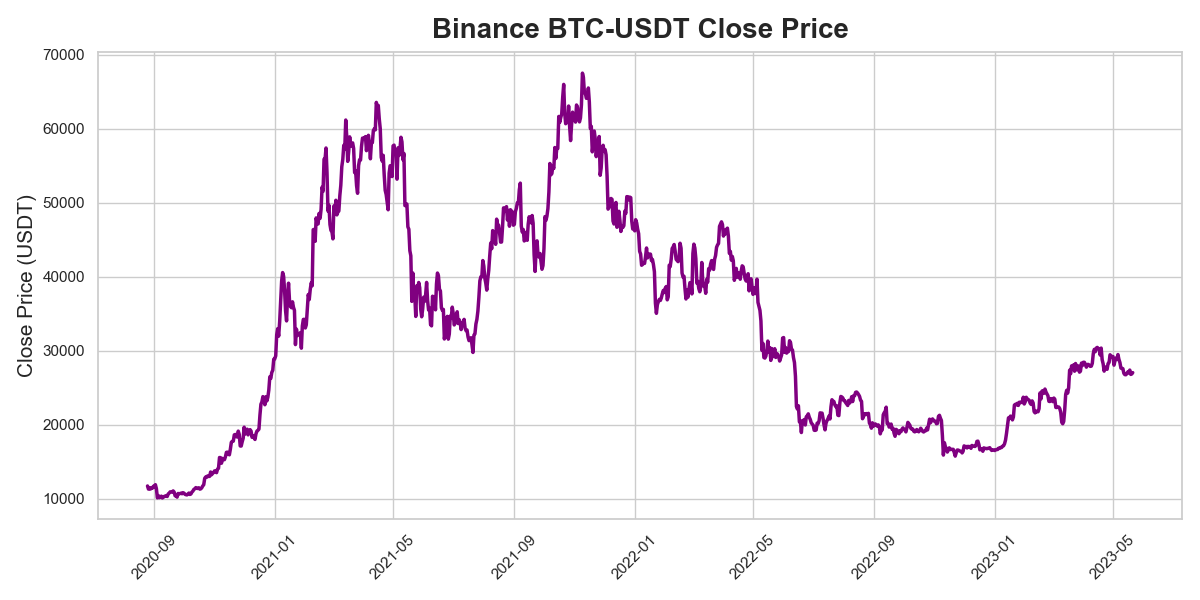
\includegraphics[width=1.0\textwidth]{Figs/BTC-USD.png}
        \caption{BTC-USD daily close prices from 23rd August 2020 to 15th May 2023 obtained from Binance. \cite{tradingview}}
        \label{fig:BTC-USD}
    \end{center}
\end{figure}

\begin{figure}[htbp]
    \begin{center}
        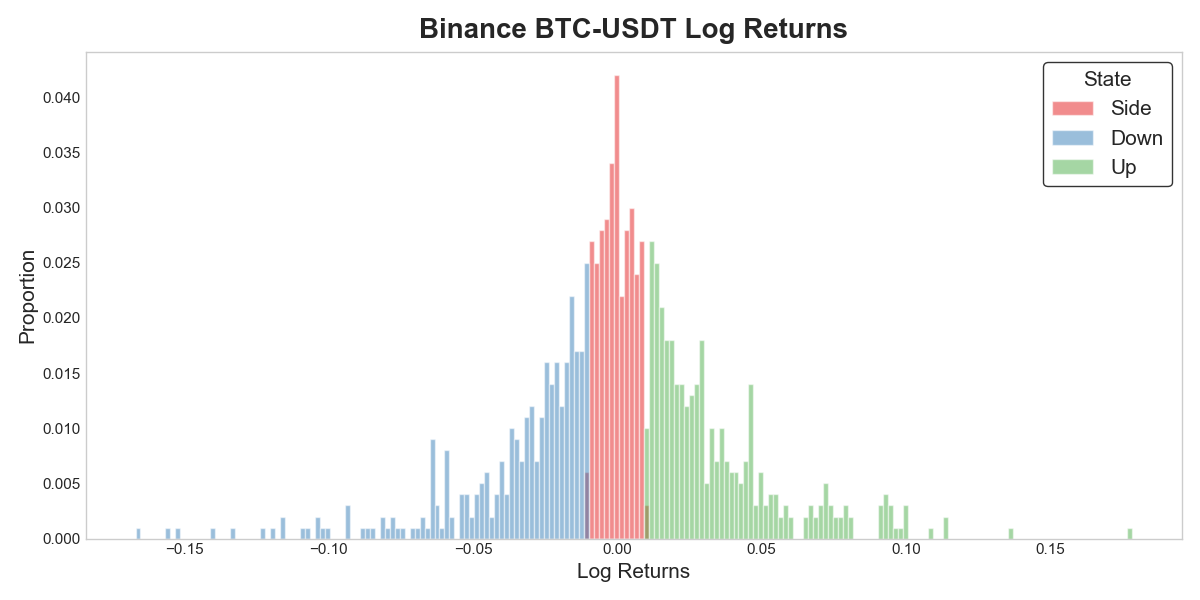
\includegraphics[width=1.0\textwidth]{Figs/BTC-USD_hist.png}
        \caption{Distribution of the log returns with respect to predefined market states. \cite{tradingview}}
        \label{fig:BTC-USD-distribution}
    \end{center}
\end{figure}

Observing the distribution of the log-returns of the daily BTC-USDT close price in \ref{fig:BTC-USD-distribution} we may conclude that such a random variable is normally distributed,
given the symmetric property of the distribution with respect to the mean value. Furthermore, it is visible that the kurtosis might be greater than 3,
which implies that the distribution has heavier tails than the normal distribution, i.e. the extreme events are more likely to occur than in the normal distribution.
Such a property is also called {\it leptokurtic} distribution which is a result of the high volatility of the cryptocurrency market.(source?)

Let us now take the ordered sample of states from the BTC-USDT close price time series data and calculate 
the transition and initial probabilities for each state as follows:

\begin{equation}
    A = \begin{pmatrix}
     0.22 & 0.16 & 0.62 \\
     0.32 & 0.27 & 0.41 \\
     0.6 & 0.19 & 0.21 \\
     \end{pmatrix}
     , \quad 
     p= \begin{pmatrix}
     0.4 & 0.19 & 0.41 \\
     \end{pmatrix}
 \end{equation}

where we note that the frequency of observing each state is proportional to the initial distribution $p$, and we assume that state space is $I = \{U,S,D\}$ 
By the definition of the transition matrix $A$, such matrix is also a stochastic matrix since it satisfies the properties given by Equation (1.5).
Each state of the transition matrix $A$ is also non-absorbing since the probability of observing a state $i$ at time $t+1$ given the state $j$ at time $t$ is greater than 0 
and aperiodic since the greatest common divisor of the lengths of all cycles in the chain is 1. Positive recurrence of each state is satisfied as well.
Furthermore, we may also conclude that the state space is irreducible since all states communicate with each other, i.e. there is a non-zero probability of transitioning from any state to any other state.
Therefore, we may conclude that the Markov Chain is ergodic, and the stationary distribution exists, is unique and is approximated by the initial distribution $p$ using Equation \ref{eq:stationary}.
Finally, we may also calculate the expected return time for each state as follows:

\begin{align}
    E[\tau_U(1)|X_0=U] &= \frac{1}{\pi_U} = \frac{1}{0.4} = 2.5 \\
    E[\tau_S(1)|X_0=S] &= \frac{1}{\pi_S} = \frac{1}{0.19} = 5.26 \\
    E[\tau_D(1)|X_0=D] &= \frac{1}{\pi_D} = \frac{1}{0.41} = 2.5
\end{align}

where $\pi$ is the stationary distribution of the Markov Chain. In other words, the expected time of returning to 
state $U$ and $D$ is 2.5 days, and 5.26 days for state $S$. Although, the expected return times provide interesting behavioral insights,
they are simplified by the Markov property of memoryless process, stock and cryptocurrency markets do have certain memory and path-dependence properties as well as they 
are effected by external factors such as news, social media, etc. Therefore, the expected return times are only approximations of the real expected return times.

%********************************** % Third Section  *************************************
\section{Continous-time Markov Chains} 

In the previous section we have considered a discrete-time Markov Chains, i.e.\ the state space and transition period was discrete. Such period means that 
the chain can stay in a state for integer number of time steps before transitioning to another state. 
For continous-time Markov Chains we will assume that the transition period is continuous, more specifically, the period is exponentially distributed with parameter $\lambda$.

Let us consider a stochastic process $\{X_t,t \geq 0\}$ with a state space $I$ and 
a distribution $\lambda$ such that for all $t \in \mathbb{R}_0^+$ and $i_0,i_1,\ldots,i_{t+1} \in I$ it holds that:

\begin{equation}
P(X_t=j|X_s=i, X_{t_n}=i_n,\ldots,X_{t_1}=i_1) = P(X_t=j|X_s=i)
\end{equation}

where $0 \leq t_1 < \ldots < t_n < s < t $ and so it is trivially seen that such expression is equivalent to the discrete-time Markov Chain property 
given by~\ref{DTMC} with the only difference of continuous transition period.

Since the state space remains the same as in discrete-time Markov Chains, we refer to the same transition matrix $A$ and initial distribution $\textbf{p}$.
In upcoming subsection, continuous-time Markov Chain is assumed to be homogeneous, i.e.\ the transition probabilities are independent of time:

\begin{equation}
p_{i,j}(s,s+t) = p_{i,j}(t), \quad i,j \in I
\end{equation}

which also implies that the transition probability is determined only by the length of the transition period $t$. 
Chapmam Kolmogorov equality for $s,t \geq 0$ also holds for continous-time Markov Chains:

\begin{equation}
p_{i,j}(s+t) = \sum_{k \in I} p_{i,k}(s) p_{k,j}(t), \quad i,j \in I
\end{equation}

Here we also assume that $\lim_{t \to 0_{+}} p_{i,j}(t) = \delta_{i,j}$ where $\delta_{i,j}$ is a Kronecker delta function, 
i.e. the transition probabilities $p_{ij}(t)$ are right continuous at $t=0$. If such condition is satisfied for any homogeneous continous-time Markov Chain, 
then the underlying stochastic process is said to be continuous and there exists its version that is separable, measurable and its trajectories are step functions almost surely. Such version allows us to infer 
certain properties of the stochastic process. 

For example, important property for such Markov Chain given Doob convergence theorem for $s \geq 0$ and $h>0$ is:

\begin{equation}
P(X_t = i, s \leq t \leq s+h|X_s=i) = \exp(-{q_i}h)
\end{equation}

which means that the probability of staying in state $i$ for time $h$ is equal to $e^{-{q_i}h}$. 
Non-negative real number $q_{i,j}$ is called {\it transition rate} from state $i$ to state $j$ and absolute transition 
rate $q_i = \sum_{j \neq i} q_{i,j}$ respectively. Trivially, in cases where the transition rate $q_i=0$, the $p_{i,i} = 1$, i.e. the state $i$ is absorbing, 
once the chain enters such state it remains in such state for infinite amount of time. On the contrary, if $0 < q_i < \infty$ then the state $i$ is non-absorbing and stable, therefore
the chain will eventually leave such a state. For infinite transition rate $q_i = \infty$ the state $i$ is called {\it unstable} where the time of staying in such state is almost surely zero.

If we consider a stable state $i$ then its expected time of staying in such state is exponentially 
distributed with expected value of $1/q_i$. In other words, the expected time of staying in state $i$ is equal 
to the inverse of the transition rate $q_i$.

Since, we have already defined that the process has exponentially distributed transition period, we may define a {\it holding time} $T_i$ as a random variable that denotes the time of staying in state $i$:

\begin{equation}
T_i = \inf \{t \geq 0 : X_t \neq i | X_0 = i\}
\end{equation}

from which it follows that $P(T_i>s) = P(X_t=i,0 \leq t \leq s|X_0=i) = e^{-q_i s}$ and its probability density functions is:

\begin{equation}
    f(x) = 
    \begin{cases}
        q_i e^{-q_i x}, & x \geq 0\\
        0, & \text{elsewhere}
    \end{cases}
\end{equation}

% is homogeneous, we may define a transition matrix $Q$ as a matrix of transition rates between each state $i,j \in I$ such that:
According to the properties of the transition rates, such time-homogeneous continuous Markov Chain should satisfy following equations:
\begin{equation}
    \begin{aligned}
    P(X_{t+h}=i|X_t=i) &= 1 - q_i h + o(h) \\
    P(X_{t+h}=j|X_t=i) &= q_{i,j} h + o(h), \quad i \neq j
    \end{aligned}
\end{equation}

where $o(h)$ is a function of $h$ such that $\lim_{h \to 0} \frac{o(h)}{h} = 0$. Let us denote $\textbf{Q}$ as transition rates matrix with entries $\{q_{i,j}: i,j \in I\}$.

Non-negative real number $q_{i,j}$ is called {\it transition rate} from state $i$ to state $j$ and absolute transition

Such intensities resemble the probability functions of Poisson process,
 and indeed homogeneous continous-time Markov Chain is a special case of Poisson process with intensity $\lambda \geq 0$ if following conditions are satisfied:

\begin{itemize}
\item [1)] Stochastic process is viewed as a jump process, i.e.\ current state $i$ either stays in state $i$ or jumps to another state $j=i+1$. Therefore, given an interval $[t,t+h]$ the probability of jumping to another state is $\lambda h + o(h)$ and the probability of staying in state $i$ is $1-\lambda h + o(h)$.
\item [2)] Intensity $\lambda$ is constant, i.e.\ the probability of jumping to another state is independent of time, i.e. depends only on the length of the interval. We refer to such process as homogeneous Poisson process.
\item [3)] Number of jumps in disjoint intervals are independent, i.e.\ the probability of jumping to another state in disjoint intervals $[t_1,t_1+h]$ and $[t_2,t_2+h]$ is equal to the probability of jumping to another state in interval $[t_1,t_1+h] \cup [t_2,t_2+h]$.
\item [4)] The probability of more than one jump in a sufficiently small interval is negligible, i.e. the probability of jumping to another state in interval $[t,t+h]$ is $o(h)$.
\item [5)] Process starts in state $i=0$ at time $t=0$.
\end{itemize}

In a case of constant return rates, the matrix $\textbf{Q}$ with entries $q_{i} = - \lambda$ and $q_{i,j} = \lambda$ as follows:

\begin{equation}
    \textbf{Q} = 
    \begin{pmatrix}
    -\lambda & \lambda & 0 & 0 & \ldots \\
    0 & -\lambda & \lambda & 0 & \ldots \\
    0 & 0 & -\lambda & \lambda & \ldots \\
    \vdots & \vdots & \vdots & \vdots & \ddots \\
    \end{pmatrix}
\end{equation}

\subsection{Cryptocurrency market movements II.}

\section{Hidden Markov Model}

Up until now we have considered visible states in a sense that the sequence of states was known, we refer to these models as $visible$ $Markov$ $Models$. In this section we will consider a situation in which we do not observe the states directly but only as a guess given other visible observations that are available to us. These "visible" observations are considered as an emissions from the hidden state sequence. Thus, the observations are assumed to be generated by the hidden states. We may interpret this relation by the following diagram where we have a hidden state sequence $Z = \{z_1,z_2,\ldots,z_T\}$:

\begin{figure}[htbp]
\begin{center}
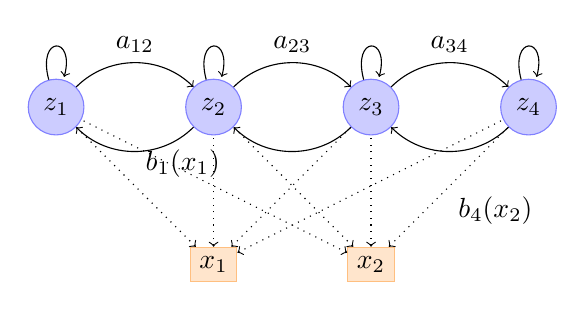
\begin{tikzpicture}[]
% states
\node[state] (s1) at (0,2) {$z_1$}
    edge [loop above]  ();
\node[state] (s2) at (2,2) {$z_2$}
    edge [<-,bend right=45] node[auto,swap] {$a_{12}$} (s1)
    edge [->,bend left=45] (s1)
    edge [loop above] ();
\node[state] (s3) at (4,2) {$z_3$}
    edge [<-,bend right=45] node[auto,swap] {$a_{23}$} (s2)
    edge [->,bend left=45] (s2)
    edge [loop above] ();
\node[state] (s4) at (6,2) {$z_4$}
    edge [<-,bend right=45] node[auto,swap] {$a_{34}$}  (s3)
    edge [->,bend left=45] (s3)
    edge [loop above] ();
% observations
\node[observation] (y1) at (2,0) {$x_1$}
    edge [lightedge] node[auto,swap] {$b_1(x_1)$} (s1)
    edge [lightedge] (s2)
    edge [lightedge] (s3)
    edge [lightedge] (s4);
\node[observation] (y2) at (4,0) {$x_2$}
    edge [lightedge] (s1)
    edge [lightedge] (s2)
    edge [lightedge] (s3)
    edge [lightedge] node[auto,swap] {$b_4(x_2)$} (s4);
\end{tikzpicture}
\end{center}
\caption{An HMM with 4 hidden states which emits 2 discrete observable states denoted by $x_1$ or $x_2$.
$a_{ij}$ is the probability to transition from state $z_i$ to state $z_j$.
$b_j(x_k)$ is the probability to emit symbol $x_k$ in state $z_j$.}
\end{figure}

There are 3 main assumptions of Hidden Markov Models as a consequence of the properties of Markov processes. For $Z = \{z_t\}_{t=0}^T$ being the hidden state sequence:

\begin{itemize}
\item[1)] The Markov assumption - this assumption states that the next hidden state $z_{t+1}$ depends only on the current state $z_t$, so that the transition probabilities are defined as:

\begin{equation}
P(z_{t+1} = j| z_{t} = i,z_{t-1} = l,\ldots,z_{0} = n) = P(z_{t+1} = j| z_{t} = i) = p_{ij}
\end{equation}

It it also possible to assume that the states in HMM are dependent beyond the current state therefore giving rise to k-order HMMs as opposed to classical first-order HMM, moreover, such variations are uneasy to analyse.

\item[2)] The stationary assumption - The transition matrix is invariant of the time, thus for any arbitrarily set time $t_1$ and $t_2$:

\begin{equation}
P(z_{t_1+1} = j| z_{t_1}) = P(z_{t_2+1} = j| z_{t_2} = i) = p_{ij}
\end{equation}

\item[3)] The observation independence assumption - The current observation or output is statistically independent of the previous observations. So if we have a observation sequence $X = \{x_1,x_2,\ldots,x_T\}$ then:

\begin{equation}
P(X|z_1,z_2,\ldots,z_T, \lambda) = \prod_{t=1}^T P(x_t|z_t,\lambda)
\end{equation}

\end{itemize}

Given these assumptions we define the joint probability of the hidden states and the observations $P(X,Z)$ as follows:

\begin{equation}
P(X, Z) = \prod_{t=1}^T P(z_t|z_{t-1}) P(x_t|z_t)
\end{equation}



There are mainly 3 fundamental problems in HMM that need to be resolved as in (Oliver C. Ibe):

\begin{itemize}
\item[1.] Evaluation problem - Given a model denoted as $\lambda = (P,\theta,\pi)$ and an observation sequence $X = x_1, x_2,\ldots,x_T$, how to efficiently compute the probability that the model generated the observation sequence, in other words, what is $P(X|\lambda)$? 
\item[2.] Decoding problem - Given a model $\lambda = (P,\theta,\pi)$, what is the most likely sequence of hidden states that could have generated a given observation sequence? Thus we would like to find $Z = \underset{Z}{\arg\max} P(Z,X|\lambda)$, where $Z$ is the hidden state sequence. 
\item[3.] The learning problem - Given a set of observation sequences find the HMM that best explains the observation sequence. Thus, find the values of $\lambda$ that maximise $P(X|\lambda)$ or in order to estimate the most likely parameters of HMM for a given observation sequence. 
\end{itemize}

The most traditional approaches in solving these 3 fundamental problems differ and one may not suffice in solving all three. The evaluation problem is usually by forward-backward algorithm, the decoding problem by well-known Viterbi algorithm and the last learning problem by Baum-Welsch algorithm which is a special case of Expectation-maximization (EM) algorithm. 

\subsection{Forward and Backward algorithm}

While given a sequence of observations, in our case observable states, denoted by $X = x_1,x_2,\ldots,x_T$ and a model $\lambda = (P,\theta,\pi)$ we wold like to compute the conditional probability of observing the sequence $X$ under the model constraints. Thus:

 \begin{equation}
P(X| \lambda) = \sum_Z P(X|Z,\lambda)*P(Z|\lambda)
\end{equation}

where $Z = z_1,z_2,\ldots,z_T$ is a fixed sequence of hidden states. Our goal may be divided into two parts while the first part $P(X|Z,\lambda)$ computes the conditional probability of the observation sequence X given the sequence Z and model $\lambda$ and the second part $P(Z|\lambda)$ accounts only for the transition probabilities among the hidden states. To summarise:

\begin{align}
P(X| Z, \lambda) &= \prod_{t=1}^T  P(x_t|z_t,\lambda) = \theta_{z_1}(x_1) \prod_{t=2}^T \theta_{z_t}(x_t) \\ \nonumber
P(Z|\lambda)&= \pi_{z_1} * \prod_{t=2}^{T} p_{z_t z_{t+1}}
\end{align}

where $\theta_{z_t}(x_t)$ is the emission probability from observation $x_t$ into $z_t$ in our model and $p_{z_t z_{t+1}}$ are the transition probabilities for the given sequence Z. After substitution of terms from Eq. 1.8 into Eq 1.7 we obtain:

\begin{align}
P(X| \lambda) &= \sum_Z P(X|Z,\lambda)*P(Z|\lambda) \\ \nonumber
&= \sum_{z_1,\ldots,z_T}\theta_{z_1}(x_1) \pi_{z_1} \prod_{t=2}^{T} p_{z_t z_{t+1}} \theta_{z_t}(x_t)
\end{align}

The summation above refers to all possible permutations of the sequence of hidden states Z which implies that we would have $N^T$ possible sequences if we assume that $N$ indicates all possible hidden states at each step. Furthermore, in order to calculate $P(X|\lambda)$ we have $2TN^T$ calculations which is exponential in T and not feasible for real application. As opposed to brute-force procedure as described above we take use of a forward and backward algorithm. 

\subsubsection{Forward algorithm}

Previous introduction required huge amounts of calculations that were essentially unnecessary, redundant. Each sequence can be decomposed into multiple subsequences which are shared among different sequences and do not need to be recomputed again. These subsequences can be represented by a trellis as shown in Fig 1.2. With a help of such diagram we may imagine recording the probability of each distinct subsequence at each time step. In other words, we wish to compute the joint probability $P(z_t,x_1,x_2,\ldots,x_t)$ while taking advantage of the conditional independence of $x_t$ which only depends on $z_t$, moreover, due to Markov assumption, $z_t$ depends only on $z_{t-1}$. Let us now define the forward probability variable $\alpha_t(i)$ as follows:

 \begin{equation}
\alpha_t(i) = P(x_1,x_2,\ldots,x_{t-1},x_t,z_t=i |\lambda)
\end{equation}

Which we may also define as the probability of being in state i at time t after having observed the sequence ${x_1,x_2,\ldots,x_t}$. The calculation therefore results in summing the incoming arcs at trellis node which is derived from:

\begin{align}
\alpha_t(i) &= P(x_1,x_2,\ldots,x_{t-1},x_t,z_t=i |\lambda) \\ \nonumber
&= P(x_t|z_t=I, \lambda) P(x_1,x_2,\ldots,x_{t-1},z_t=i |\lambda)  \\ \nonumber
&= P(x_t|z_t=i, \lambda) \sum_{j \in I} P(z_t = I| z_{t-1}=j,\lambda) P(x_1,x_2,\ldots,x_{t-1},z_{t-1}=j |\lambda) \\ \nonumber
&= \theta_i(x_t) \sum_{j=1}^N p_{ji} \alpha_{t-1}(j)
\end{align}

Where $I$ is a set of all possible hidden states, $i,j$ denote elements of $I$ and $N$ the size of set $|I|$. We would repeat the iterative procedure until the termination at time T where $P(X|\lambda) = \sum_{i=1}^N  \alpha_T(i) = \sum_{i=1}^N P(X,z_T=I|\lambda)$. Moreover, we initialise the trellis with $\alpha_1(i)=\pi_i \theta_i(x_1)$. Resulting algorithm requires time complexity of $O(TN^2)$ which is a significant improvement from the brute force approach with complexity of $O(2TN^T)$.
  
\begin{figure}[htbp]
\begin{center}
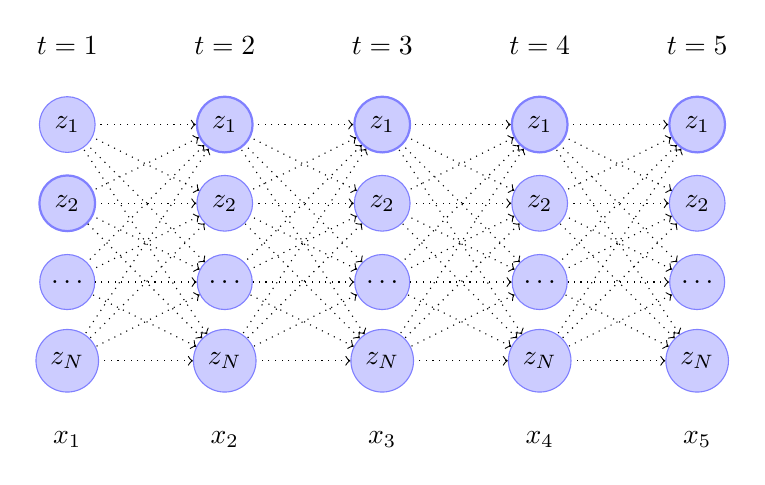
\begin{tikzpicture}[]
% 1st column
\node               at (0,6) {$t=1$};
\node[state] (s1_1) at (0,5) {$z_1$};
\node[mainstate] (s2_1) at (0,4) {$z_2$};
\node[state] (s3_1) at (0,3) {$\ldots$};
\node[state] (s4_1) at (0,2) {$z_N$};
\node at (0,1) {$x_1$};
% 2nd column
\node               at (2,6) {$t=2$};
\node[mainstate] (s1_2) at (2,5) {$z_1$}
    edge[lightedge] (s1_1)
    edge[lightedge] (s2_1)
    edge[lightedge] (s3_1)
    edge[lightedge] (s4_1);
\node[state] (s2_2) at (2,4) {$z_2$}
    edge[lightedge] (s1_1)
    edge[lightedge] (s2_1)
    edge[lightedge] (s3_1)
    edge[lightedge] (s4_1);
\node[state] (s3_2) at (2,3) {$\ldots$}
    edge[lightedge] (s1_1)
    edge[lightedge] (s2_1)
    edge[lightedge] (s3_1)
    edge[lightedge] (s4_1);
\node[state] (s4_2) at (2,2) {$z_N$}
    edge[lightedge] (s1_1)
    edge[lightedge] (s2_1)
    edge[lightedge] (s3_1)
    edge[lightedge] (s4_1);
\node at (2,1) {$x_2$};
% 3rd column
\node               at (4,6) {$t=3$};
\node[mainstate] (s1_3) at (4,5) {$z_1$}
    edge[lightedge]  (s1_2)
    edge[lightedge] (s2_2)
    edge[lightedge] (s3_2)
    edge[lightedge] (s4_2);
\node[state] (s2_3) at (4,4) {$z_2$}
    edge[lightedge] (s1_2)
    edge[lightedge] (s2_2)
    edge[lightedge] (s3_2)
    edge[lightedge] (s4_2);
\node[state] (s3_3) at (4,3) {$\ldots$}
    edge[lightedge] (s1_2)
    edge[lightedge] (s2_2)
    edge[lightedge] (s3_2)
    edge[lightedge] (s4_2);
\node[state] (s4_3) at (4,2) {$z_N$}
    edge[lightedge] (s1_2)
    edge[lightedge] (s2_2)
    edge[lightedge] (s3_2)
    edge[lightedge] (s4_2);
\node at (4,1) {$x_3$};
% 4th column
\node               at (6,6) {$t=4$};
\node[mainstate] (s1_4) at (6,5) {$z_1$}
    edge[lightedge]  (s1_3)
    edge[lightedge] (s2_3)
    edge[lightedge] (s3_3)
    edge[lightedge] (s4_3);
\node[state] (s2_4) at (6,4) {$z_2$}
    edge[lightedge] (s1_3)
    edge[lightedge] (s2_3)
    edge[lightedge] (s3_3)
    edge[lightedge] (s4_3);
\node[state] (s3_4) at (6,3) {$\ldots$}
    edge[lightedge] (s1_3)
    edge[lightedge] (s2_3)
    edge[lightedge] (s3_3)
    edge[lightedge] (s4_3);
\node[state] (s4_4) at (6,2) {$z_N$}
    edge[lightedge] (s1_3)
    edge[lightedge] (s2_3)
    edge[lightedge] (s3_3)
    edge[lightedge] (s4_3);
\node at (6,1) {$x_4$};
% 5th column
\node               at (8,6) {$t=5$};
\node[mainstate] (s1_5) at (8,5) {$z_1$}
    edge[lightedge]  (s1_4)
    edge[lightedge] (s2_4)
    edge[lightedge] (s3_4)
    edge[lightedge] (s4_4);
\node[state] (s2_5) at (8,4) {$z_2$}
    edge[lightedge] (s1_4)
    edge[lightedge] (s2_4)
    edge[lightedge] (s3_4)
    edge[lightedge] (s4_4);
\node[state] (s3_5) at (8,3) {$\ldots$}
    edge[lightedge] (s1_4)
    edge[lightedge] (s2_4)
    edge[lightedge] (s3_4)
    edge[lightedge] (s4_4);
\node[state] (s4_5) at (8,2) {$z_N$}
    edge[lightedge] (s1_4)
    edge[lightedge] (s2_4)
    edge[lightedge] (s3_4)
    edge[lightedge] (s4_4);
\node at (8,1) {$x_5$};
\end{tikzpicture}
\end{center}
\caption{Trellis of the observation sequence $x_1$,\ldots,$x_5$ for the above HMM.\@ As an example, the transition between state $z_1$ at time t=2 and state $z_4$ at time t=3 has probability $\alpha_2(z_1)p_{14}\theta_{z_4}(x_3)$, where $\alpha_t(i)$ is the probability to be instate $i$ at time t.}
\end{figure}

\pagebreak

\subsubsection{Backward algorithm}

While computing the backward probability variable denoted as $\beta_t(i)$ we assume the reversed iterative procedure. Let us define the backward probability variable as:

\begin{align}
\beta_t(i) &= P(x_{t+1},x_{t+2},\ldots,x_{t-1},x_t|z_t=i ,\lambda) \\ \nonumber
&= \sum_{i,j \in I} P(x_{t+1},x_{t+2},\ldots,x_{t-1},x_t,z_{t+1}=j|z_t=i ,\lambda)   \\ \nonumber
&= \sum_{i,j \in I} P(x_{t+1}|z_{t+1}=j) P(x_{t+2},\ldots,x_{t-1},x_t|z_{t+1}=j) P(z_{t+1}=j|z_{t}=i,\lambda) \\ \nonumber
&= \sum_{j=1}^N \theta_j(x_{t+1})p_{ij} \beta_{t+1}(j)
\end{align}

As we could have in forward algorithm we define effectively 3 steps:

\begin{itemize}
\item[1.] Initialization step: with default value of $\beta_T(i) = 1$ for $i \in {1,2,\ldots,N}$. 
\item[2.] Induction step: 

\begin{equation}
\beta_t(i) = \theta_j(x_{t+1})p_{ij} \beta_{t+1}(j)
\end{equation}

Afterwards, we update the time t = t-1 and check whether expression above holds which is as long as t $>$ 0.
\item[3.] Termination step: once the iterative procedure is exhausted, i.e.\ when t=0 we have the estimate of $P(X|\lambda)$ as:

\begin{equation}
P(X|\lambda) = \sum_{j=1}^N \theta_j(x_{1})\pi_{i} \beta_{1}(i) = \sum_{j=1}^N \alpha_1(i)  \beta_{1}(i)
\end{equation}

\end{itemize}

Getting everything together we may prove that the forward and backward algorithms coincide in solving the posterior joint and marginal distributions of all hidden states. Consider the case of posterior joint distribution:

\begin{align}
P(X|\lambda) &= \sum_{i=1}^N P(X,z_t=i|\lambda) \\ \nonumber
&= \sum_{i=1}^N P(x_1,x_2,\ldots,x_{t},x_{t+1},\ldots,x_{T}|z_t=i,\lambda) P(z_t = i|\lambda) \\ \nonumber
&= \sum_{i=1}^N P(x_1,x_2,\ldots,x_{t}|z_t=i,\lambda) P(x_{t+1},\ldots,x_{T}|z_t=i,\lambda) P(z_t = i|\lambda) \\ \nonumber
&= \sum_{i=1}^N P(x_1,x_2,\ldots,x_{t},z_t=i|\lambda) P(x_{t+1},\ldots,x_{T}|z_t=i,\lambda) \\ \nonumber
&= \sum_{i=1}^N \alpha_{t}(i) \beta_t(i) 
\end{align}

See that above we take a use of conditional independence of observations given the hidden state and therefore we may transform the problem using already known variables for forward and backward passes over the hidden states. Thus, the posterior marginal distribution is:

\begin{equation}
P(X, z_t=i|\lambda) = \alpha_t(i) \beta_t(i)
\end{equation}

\subsection{Viterbi algorithm}

Once we solve the evaluation problem, thus finding the optimal procedure in computing the posterior marginal distributions of all hidden states and $P(X|\lambda)$, we may visualise the result in a trellis as shown in Figure 1.2. The second problem, decoding problem, aims to find the sequence of hidden states $Z^*$ that most likely produced observation sequence $X$. Finding the most likely sequence $Z^*$ maximazes $P(Z|X,\lambda)$. As in the encoding problem, the complexity of the optimisation problem explodes if we decide to compute all possible sequences of hidden states to $N^T$ calculations. The solution as in the forward and backward algorithm simplifies when we calculate the hidden state with highest probability individually rather than entire sequence up to time $t$. The idea is that once we find the most likely hidden state given observation and the model at each time step we may discard the rest of the possible hidden states since they obviously could not have most likely produced the observation. The complexity of the optimal sequence of hidden states decreases significantly to $NT$ thus transforming the exponential complexity into linear. As in forward and backward algorithm we define variable $\gamma_t(i)$ as:

\begin{equation}
\gamma_t(i) = P(z_t=i|X,\lambda) = \frac{P(X,z_t=i|\lambda)}{P(X|\lambda)} =\frac{\alpha_t(i) \beta_t(i)}{\sum_{i=1}^N \alpha_t(i) \beta_t(i)} \propto \alpha_t(i) \beta_t(i)
\end{equation}

Where the expressions in the third equality are obtained as a solution to a before mentioned equations. Also, the $P(X|\lambda)$ serves only as a normalising constant and is irrelevant for the optimisation given the respective time step. Moreover, the conditional probability $\gamma_t(i)$ forms a conditional probability mass function since it is non-negative for all possible values of hidden states and observations and the sum over all possible hidden states at each time step is:

\begin{equation}
\sum_{i=1}^N  \gamma_t(i) = 1
\end{equation}

This would be one of the possible ways to estimate the most likely hidden states individually and then combine them sequentially to obtain the whole sequence of hidden states as:

\begin{equation}
z_t^* = \underset{i \in I}{\arg\max} \{\gamma_t(i)\}
\end{equation}

Method as described by the Eq 1.17 and 1.19 is also called maximum a posteriori probability estimate (hereinafter `MAP estimate`) which equals to the mode of the posterior distribution. If the posterior distribution is discrete, the mode is simply the value of a random variable with the highest probability. For continuous distributions the mode is a value of a random variable for which the likelihood/log-likelihood function attains its local maximum/maxima. Assuming now $Z$ denotes the continuous random variable of hidden states and observation sequence $X$ up to time t is present, the MAP estimate of the hidden state $\hat{Z}_{MAP}$ at a given point in time is:

\begin{align}
\hat{z}_{t,MAP} &= \underset{z_t}{\arg\max} \: f(Z_t|X) \\ \nonumber
&= \underset{z_t}{\arg\max} \: \frac{f(X|Z_t)g(Z_t)}{\int_{I} f(X|Z_t)g(Z_t) \,dZ} \\ \nonumber
&= \underset{z_t}{\arg\max} \: f(X|Z_t)g(Z_t)\\ \nonumber
\end{align}

Where $g$ indicates probability density function of $Z_t$, so called prior distribution, and $I$ is its domain. The second equality follows from the Bayes' Theorem. The result clearly holds for the discrete case:

\begin{align}
\hat{z}_{t,MAP} &= \underset{z_t}{\arg\max} \: P(Z_t=i|X) \\ \nonumber
&= \underset{z_t}{\arg\max} \: \frac{P(X|Z_t=i)P(Z_t=i)}{\sum_{i=1}^N P(X|Z_t=i)P(Z_t=i)} \\ \nonumber
&= \underset{z_t}{\arg\max} \:P(X|Z_t=i)P(Z_t=i)\\ \nonumber
&= z_t^*\\ \nonumber
\end{align}

However, the solution as such might not produce the most likely sequence of states given the sequence of observations. This is due to the fact that the individual estimates do not incorporate the transition probability between most likely states at time t-1 and t. Hence, it might be possible that some states are highly unlikely to transition into other that were evaluated as most likely. Fortunately, the mentioned shortcomings of such approach are easily solved by Viterbi algorithm.

In order to find the most likely sequence of hidden states $Z^*={z_1^*,z_2^*,\ldots,z_T^*}$ given the observation sequence $X={x_1,x_2,\ldots,x_T}$ it is necessary to maximise with respect to the whole sequence rather than individually to avoid less likely transitions as introduced. The algorithm therefore defines a variable as follows:

\begin{equation}
\delta_t(i) = \underset{Z_{t-1}}{\max}\:P(z_1,z_2,\ldots,z_t=i,x_1,x_2,\ldots,x_{t-1},x_{t}|\lambda)
\end{equation}

That is the most likely state sequence given the observation sequence up to time $t$. Moreover, for the purpose of the algorithm we also define variable $\psi_t(i)$ that stores the node of the incoming arc that leads to the most probable state path.

\begin{equation}
\psi_t(j) = \underset{i \in I}{\arg\max} \: \delta_{t-1}(i)p_{ij}
\end{equation}

\vspace{0.3cm}

\noindent
Then we can easily provide the steps to obtain the most likely state sequence:

\begin{itemize}
\item[1.] Initialize the algorithm given the initial distribution of hidden states $\pi$:

\begin{align}
\delta_1(i) &= \pi_i b_i(o_1)  \\
\psi_1(i)& = 0
\end{align}

where we compute the initial values of above variables for each hidden state $i \in I$.

\item[2.] Recursive step:

\begin{align}
\delta_1(i) &= \underset{i \in I}{\arg\max} \: \delta_{t-1}(i)p_{ij} b_j(o_t)  \\
\psi_t(j)& = \underset{i \in I}{\arg\max} \: \delta_{t-1}(i)p_{ij}
\end{align}

At each iterative step we update the time so that $t=t+1$. The second step continues as long as the $t<T$ if that does not hold the third step terminates the algorithm and we backtrack the most likely state sequence. Although, recursive step is very similar to the induction step in the forward algorithm there exist a main difference between the two that lies in the fact that Viterbi algorithm uses maximization instead of summation over previous states. 

\item[3.] Termination step for the last observation 

\begin{align}
P^* &= \underset{i \in I}{\max} \: \delta_{T}(i) \\
q_T^* & = \underset{i \in I}{\arg\max} \: \delta_{T}(i)
\end{align}

\item[4.] Backtrack the optimal state sequence:

\begin{equation}
z_t^* = \psi_{t+1}(z_{t+1}^*)
\end{equation}

For $t = T-1,T-2,\ldots,1$.

\end{itemize}

The resulting most likely state path can be visually viewed as in the form of a path within the trellis introduced in Fig. 1.2:

\begin{figure}[htbp]
\begin{center}
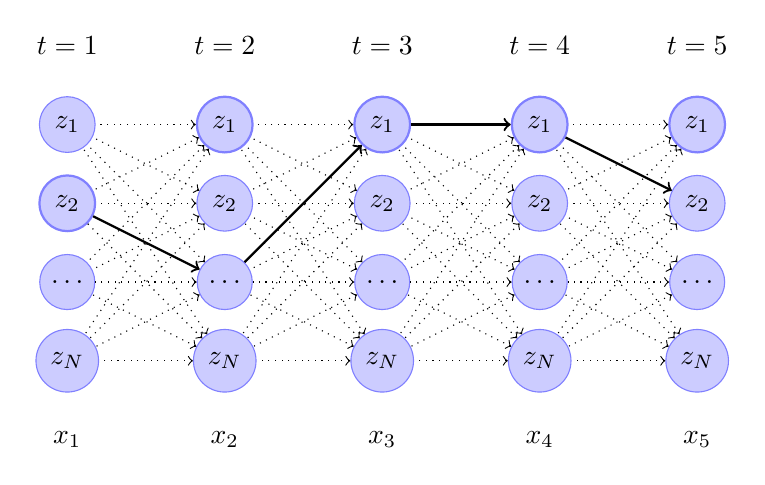
\begin{tikzpicture}[]
% 1st column
\node               at (0,6) {$t=1$};
\node[state] (s1_1) at (0,5) {$z_1$};
\node[mainstate] (s2_1) at (0,4) {$z_2$};
\node[state] (s3_1) at (0,3) {$\ldots$};
\node[state] (s4_1) at (0,2) {$z_N$};
\node at (0,1) {$x_1$};
% 2nd column
\node               at (2,6) {$t=2$};
\node[mainstate] (s1_2) at (2,5) {$z_1$}
    edge[lightedge] (s1_1)
    edge[lightedge] (s2_1)
    edge[lightedge] (s3_1)
    edge[lightedge] (s4_1);
\node[state] (s2_2) at (2,4) {$z_2$}
    edge[lightedge] (s1_1)
    edge[lightedge] (s2_1)
    edge[lightedge] (s3_1)
    edge[lightedge] (s4_1);
\node[state] (s3_2) at (2,3) {$\ldots$}
    edge[lightedge] (s1_1)
    edge[mainedge] (s2_1)
    edge[lightedge] (s3_1)
    edge[lightedge] (s4_1);
\node[state] (s4_2) at (2,2) {$z_N$}
    edge[lightedge] (s1_1)
    edge[lightedge] (s2_1)
    edge[lightedge] (s3_1)
    edge[lightedge] (s4_1);
\node at (2,1) {$x_2$};
% 3rd column
\node               at (4,6) {$t=3$};
\node[mainstate] (s1_3) at (4,5) {$z_1$}
    edge[lightedge]  (s1_2)
    edge[lightedge] (s2_2)
    edge[mainedge] (s3_2)
    edge[lightedge] (s4_2);
\node[state] (s2_3) at (4,4) {$z_2$}
    edge[lightedge] (s1_2)
    edge[lightedge] (s2_2)
    edge[lightedge] (s3_2)
    edge[lightedge] (s4_2);
\node[state] (s3_3) at (4,3) {$\ldots$}
    edge[lightedge] (s1_2)
    edge[lightedge] (s2_2)
    edge[lightedge] (s3_2)
    edge[lightedge] (s4_2);
\node[state] (s4_3) at (4,2) {$z_N$}
    edge[lightedge] (s1_2)
    edge[lightedge] (s2_2)
    edge[lightedge] (s3_2)
    edge[lightedge] (s4_2);
\node at (4,1) {$x_3$};
% 4th column
\node               at (6,6) {$t=4$};
\node[mainstate] (s1_4) at (6,5) {$z_1$}
    edge[mainedge]  (s1_3)
    edge[lightedge] (s2_3)
    edge[lightedge] (s3_3)
    edge[lightedge] (s4_3);
\node[state] (s2_4) at (6,4) {$z_2$}
    edge[lightedge] (s1_3)
    edge[lightedge] (s2_3)
    edge[lightedge] (s3_3)
    edge[lightedge] (s4_3);
\node[state] (s3_4) at (6,3) {$\ldots$}
    edge[lightedge] (s1_3)
    edge[lightedge] (s2_3)
    edge[lightedge] (s3_3)
    edge[lightedge] (s4_3);
\node[state] (s4_4) at (6,2) {$z_N$}
    edge[lightedge] (s1_3)
    edge[lightedge] (s2_3)
    edge[lightedge] (s3_3)
    edge[lightedge] (s4_3);
\node at (6,1) {$x_4$};
% 5th column
\node               at (8,6) {$t=5$};
\node[mainstate] (s1_5) at (8,5) {$z_1$}
    edge[lightedge]  (s1_4)
    edge[lightedge] (s2_4)
    edge[lightedge] (s3_4)
    edge[lightedge] (s4_4);
\node[state] (s2_5) at (8,4) {$z_2$}
    edge[mainedge] (s1_4)
    edge[lightedge] (s2_4)
    edge[lightedge] (s3_4)
    edge[lightedge] (s4_4);
\node[state] (s3_5) at (8,3) {$\ldots$}
    edge[lightedge] (s1_4)
    edge[lightedge] (s2_4)
    edge[lightedge] (s3_4)
    edge[lightedge] (s4_4);
\node[state] (s4_5) at (8,2) {$z_N$}
    edge[lightedge] (s1_4)
    edge[lightedge] (s2_4)
    edge[lightedge] (s3_4)
    edge[lightedge] (s4_4);
\node at (8,1) {$x_5$};
\end{tikzpicture}
\end{center}
\caption{Trellis of the observation sequence $x_1$, \ldots,$x_5$ for the HMM.\@ Bold lines illustrate the most likely sequence found by the Viterbi algorithm.}
\end{figure}


\newpage

\section{Kalman Filters}
